\section{Referee 3}\label{ref3}
\RC The paper studies Bayesian D-optimal design (that is, the task of
allocating measurements in order to maximise the Kullback-Leibler
divergence between the prior and posterior distribution) in an inverse
regression type model in Hilbert spaces with Gaussian measurements
errors. For Gaussian priors, the paper provides a characterisation of
the optimality criterion and the optimal design. Some conclusions
about the phenomenon of clusterisation of measurements known in
literature are then drawn.


\RC While the results in the paper provide some novel insights on the
topic, I believe the current version of the manuscript is far from the
standard required by Bayesian Analysis. Let me raise immediately my
main concern: on p.4 the author describes the generality of
measurements clusterisation as the first main question being explored,
which is answered via, quoting, "randomized numerical simulations that
exhibit clusterization more than 95\% of the time (see the code in
supplementary material)". However, in the version of the supplementary
materials I had access to there is no further mention of these
numerical simulations and results; only a link to a Github repository
is provided, which is however not functioning.

\AR I made sure the repository is functioning and well-documented. See
\url{https://github.com/yairdaon/OED}. Furthermore, I added references
to specific modules in the text, see excerpts below.

\begin{quote}
Full results are located in the \texttt{simulations.csv} file within
the accompanying \href{https://github.com/yairdaon/OED}{repository}.
Code implementing the experiments described above is located in module
\texttt{zeros.py} of said repository.
\end{quote}
\begin{quote}
Code generating these movies is located in module \texttt{movies.py}
in the accompanying
\href{https://github.com/yairdaon/OED}{repository}.
\end{quote}
\begin{quote}
The implementation of the D-optimality criterion for this inverse
problem with homogeneous Neumann and Dirichlet boundary conditions can
be found in directory \texttt{src/} and script
\texttt{clusterization.py} in the accompanying
\href{https://github.com/yairdaon/OED}{repository}.
\end{quote}


\RC Evidently, this issue needs to be fixed before any future
consideration can be given to the manuscript. For example, a detailed
description of the repeated experiments could be provided either in
the main article or in the supplement, with tables indicating the
various values of the parameters for the simulations and the precise
percentages obtained. Also, the code needs to be publicly available
for reproducibility.

\AR I appreciate the suggestion. I added a section reproducing the
abovementioned numerical experiments to the main article. See Section
\ref{subsec:lemma_sims} reproduced below:


\begin{quote} %% Simulate
  In the proof of Theorem \ref{thm:char} we utilize Lemma
\ref{lemma:free} to construct D-optimal designs. We implement this
construction with the goal of testing numerically how prevalent are
clustered designs. To this end, we would like to generate random prior
eigenvalues $\lambda_j$, fix $m$ and $k$, find what a D-optimal
$\opt^*\opt$ should be, and then utilize the construction of
Theorem~\ref{thm:char} and Lemma~\ref{lemma:free} to find $\opt$.


To simplify things, we directly generate $\opt^*\opt$. We iterate over
the number of measurements $m \in \{4,\dots, 24\}$, and for every $m$
we then iterate over $k:=\rank \opt^*\opt \in \{2,\dots, m-1\}$. For
each pair $m,k$ we repeat the following steps $N=5000$ times:
\begin{enumerate}
\item Generate random diagonal $D\in \mathbb{R}^{k\times k}$ with
  entries $\log (d_i) \sim \mathcal{N}(50,15)$.
\item Normalize $D$ that $\ttr D = m$.
\item Conjugate $D$ by a random orthogonal matrix to form a positive
  semi-definite $M := UDU^t \in \mathbb{R}^{k\times k}$. This $M$
  represents $\opt^*\opt$.
\item Apply the construction of Lemma \ref{lemma:free} to calculate
  $A$ such that $AA^t = M$, where $A$ has unit norm columns. $A^t$ is
  our optimal design $\opt$.
\item Since $A^t$ corresponds to $\opt$, its columns correspond to
  measurement vectors. We call $A$ "clustered" if $A$ has two or more
  identical columns (up to some numerical precision threshold,
  i.e.~$10^{-5}$).
\end{enumerate}
We then calculate the fraction of clustered designs of the simulations
we ran, for each pair $m,k$. Clusterization occurred at high rates
($>99.9\%$) whenever $m-k > 1$; see Fig.~\ref{fig:sim_AAt}. Hence, in
these simulations, clusterization is a generic property. However, when
$m-k = 1$, clusterization does not occur. We do not why this is so.
\newline
\newline
Full results are located in the \texttt{simulations.csv} file within
the accompanying \href{https://github.com/yairdaon/OED}{repository}.
Code implementing the experiments described above is located in module
\texttt{zeros.py} of said repository. Runtime should be less than 30
minutes on any reasonably modern laptop (it took 12 minutes on the
author's laptop).
\end{quote}

\begin{figure}
    \centering
    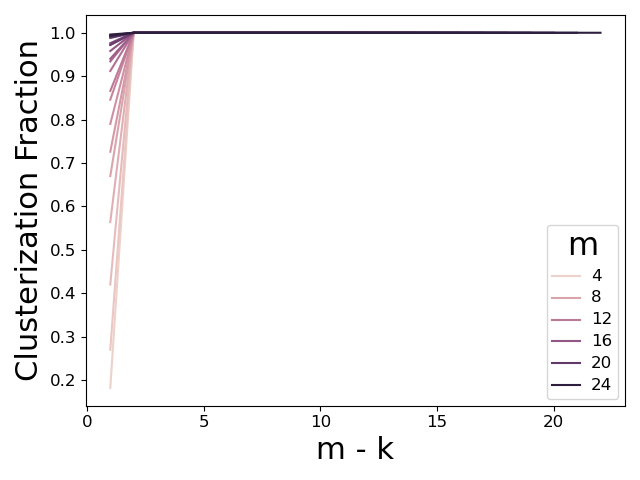
\includegraphics[height=0.5\textwidth]{../latex/figs/simulations.png}
    \caption{Fraction of clustered $A$ for $AA^t = M$ and $M$
      generated randomly (see text and repository for details on
      generating $M$). It is evident that when $m-k > 1$ clusterization
      is prevalent, whereas for lower $m-k$ clusterization is not.}
  \label{fig:sim_AAt}
\end{figure}

\subsection{Further comments}
\RC I have a number of further comments in regards to the results and the
overall presentation of the manuscript.


\RC D-optimal design vs. statistical recovery rates: being more
familiar with the statistical inverse problem literature than with
D-optimal design, the clusterisation phenomenon demonstrated in this
paper raises the question as to whether consistent recovery of the
unknown ($\param$ in the notation of this paper) is possible under
this choice. All the results I am aware of either assume white
noise/equally spaced design (e.g.~\cite{knapik2011}) or measurement
locations sampled uniformly at random (e.g.~\cite{nickl2023}). There
are also some results with more general design under conditions on the
fill-distance of the grid (e.g.~\cite{teckentrup2020}). All of these
specifically prevent clusterisation, which is key to the statistical
analysis. Hence, it is not clear to me even if D-optimal design should
be pursued at all, if it indeed it leads to clusterisation as implied
by the present paper. I think a discussion on this would be
illuminating for the reader and help draw a connection to the broader
statistical inverse problems literature.

\AR I added a discussion on this subject. In the manuscript this
discussion is broken in two since the second part relies on Theorem
\ref{thm:char}. Thus, the first part is in the Introduction and the
second part follows the statement and proof of the abovementioned
theorem.
\begin{quote}%%Convergence
  Clusterization in D-optimal designs raises the question of whether
  D-optimal designs should be pursued at all. While other authors have
  established convergence results for decaying measurement error
  \cite{knapik2011}, space-filling measurements \cite{teckentrup2020}
  and randomly sampled designs \cite{nickl2023}, their results do not
  hold for D-optimal designs. Luckily, we can expect convergence from
  D-optimal designs (including clustered designs) in the following
  sense: the posterior uncertainty ellipsoid will contract to zero
  along each one of its eigenvectors. See Section
  \ref{subsub:convergence} for a precise statement and a proof based
  on Theorem \ref{thm:char} --- the main theorem of this manuscript.
\end{quote}
\begin{quote}
  In this section we fulfill our promise from Section
  \ref{subsub:implications} and prove that the posterior uncertainty
  ellipsoid in $\hilo$ will contract to zero along every eigenvector
  of $\fwd \prcov \fwd^*$. In our proof we ignore potential problems
  with conducting inference on function spaces which are not unique to
  D-optimal designs (see e.g.~\cite{owhadi2015} for more details).
  \newline
  \newline  
  First, denote $\opt_m$ a D-optimal design utilizing $m$ measurements
  and denote $k_m := \rank\opt_m^*\opt_m$. An immediate consequence of
  Theorem \ref{thm:char} is that allowing more measurements will
  eventually allow us to measure each eigenvalue, i.e.:
  \begin{equation}\label{eq:lim}
    \lim_{m\to\infty} k_m = \infty
  \end{equation}
  \newline
  \newline
  Now, recall that part (5) of Theorem \ref{thm:char} ensures that the
eigenvalues of the posterior pushforward covariance equal
\begin{equation*}
  \theta^{(k)}_i = \left ( \frac{\sum_{j=1}^{k} \lambda_j^{-1} +
    \sigma^{-2}m}{k} \right )^{-1}, \text{ for $i\leq k$}.
\end{equation*}
Using the inequality for the arithmetic and harmonic means, it is easy
to verify that
\begin{equation*}
  \theta^{(k)}_i \leq \lambda_{k}.
   %% \leq \frac{\sum_{j=1}^{k} \lambda_j}{k}
\end{equation*}
Since $\lim_{k\to \infty} \lambda_k= 0$, we conclude that for all $i$,
$\lim_{k\to\infty} \theta^{(k)}_i = 0$. Combining the latter
observation with eq.~\eqref{eq:lim}, we conclude that
$\lim_{m\to\infty} \theta^{(k_m)}_i = 0$ for all $i$. Therefore,
posterior uncertainty decays to zero for all eigenvectors.
\end{quote}




\RC Figure 1: It is hard to discern whether the measurements locations
are perfectly overlapping or just very closely placed. Perhaps using
dots with numbers here would help the readability.
  
\AR It is impossible to visually discern the measurements, even when
resolution is increased. These measurements are not identical
numerically, but they are identical to five decimal digits. Since I
find these points via optimization over point location in
$\Omega=[0,1]$ I view a numerical error $<10^{-5}$ as reasonable.

\RC Experiment with the 1D heat equation: the experiment showcases
some interesting phenomena, but also raises many questions. For
instance: I would expect the dimensionality of the working domain
(here the unit interval $[0, 1]$) to play a role, since larger
dimension allow for higher freedom in placing the design points.
Further, a dimensionality effect should also arise directly from
Theorem 1\footnote{Now denoted Theorem \ref{thm:char}.} via the prior
covariance eigenvalues: in the experiment the prior covariance
operator is set to be equal to the inverse Laplace operator
$(-\Delta)^{-1}$. In d-dimensional domains, its eigenvalues
$\lambda_j$ are known to follow Weyl’s asymptotics, growing as
$j^{2/d}$, which should then impact the index after which the
eigenvalues are ‘thresholded’ by the procedure.

\AR These are two great points. Indeed, the growth of eigenvalues of
the Laplacian is different in higher dimensions. This is why in higher
dimensions we would have to take as prior \(u_0 \sim
\mathcal{N}(\param_0, (-\Delta)^{-\gamma})\), for some \(\gamma >
d/2\) in order to maintain regularity of prior realizations. I decided
not to include a discussion on the choice of priors in higher spatial
dimensions because (1) it would require too much exposition and make
me digress from the main points I wanted to convey and (2) due to
technical difficulties in installing packages for inverse problems
\cite{attia2023pyoed, villa18} I had to implement the inverse problem
of the 1D heat equation from scratch, so I decided to leave out
experiments in higher dimensions.

  
\RC Also, it should be relatively easy here to also study empirically
the effect of the correlated error model in preventing
clusterisation. Investigating all these issues in the context of the
presented numerical set up would considerably enlarge the breath of
the present work.

\AR I added relevant simulations to a new section Numerical
Experiments:


\begin{quote}
  In order to verify the results of Section
  \ref{section:non_vanishing}, we run simulations of the inverse
  problem of the 1D heat equation with nonvanishing model error
  \(\modcov = \prcov^2 \). Indeed, including model correlation pushes
  measurements apart, see Fig.~\ref{fig:corr_errors}. Code generating
  Fig.~\ref{fig:corr_errors} is located in module
  \texttt{clusterization.py} in the accompanying
  \href{https://github.com/yairdaon/OED}{repository}.
\end{quote}
\begin{figure}
  \centering
  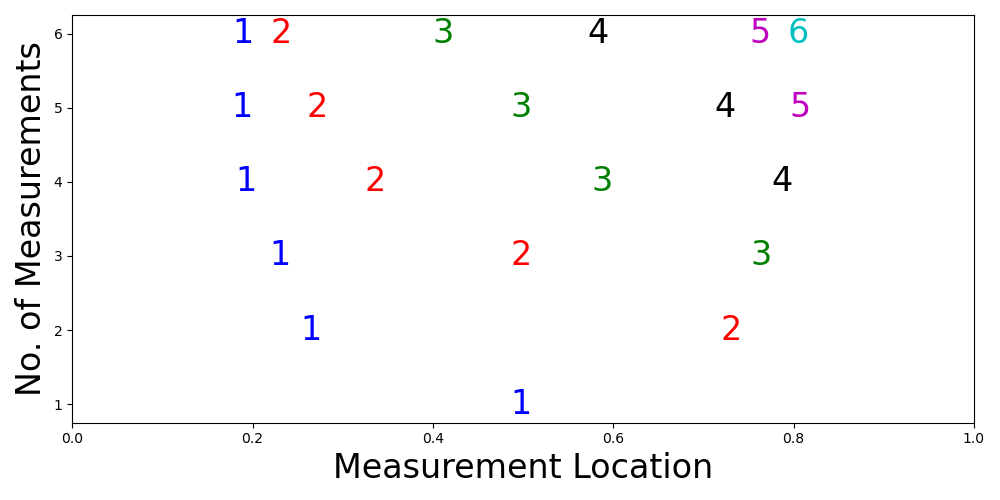
\includegraphics[height=0.5\textwidth]{../latex/figs/dst_modelError4.png}
  \caption{Model correlation mitigates clusterization. We add a
    model correlation term to the error terms in the 1D heat
    equation inverse problem. Lo and behold, measurements are not
    close anymore and are pushed away thanks to the model error
    term.}
    \label{fig:corr_errors}
\end{figure}

  
\RC I found very hard to understand Theorem 1 immediately at the end
of Section 1, as all the necessary background is introduced only
later. Since the same result is also stated and proved in Section 5, I
would consider cutting it from Section 1. The paragraphs in p.4 and 5
already do a good job presenting the results, and the repetition of
the formal statement does not seem necessary here.

\AR I removed the statement of Theorem 1 from the Introduction. It is
Theorem \ref{thm:char} now.


\RC Denoting the optimal design in Theorem 1 by simply $\obs$ is
somewhat confusing, cf.~the equation in the second item. Perhaps a
separate notation such as $\bar{\obs}$ would help readability.

\AR Thank you for the comment, I completely agree. Optimal designs are
now denoted $\opt$.

  
\RC Section 1.2 seems altogether unnecessary; the inverse regression
model considered in the paper are a modelisation of many real-world
phenomena, and they are routinely studied in statistical papers.

\AR I am glad you view this part as unnecessary, but I feel the model
might feel too abstract to some practitioners. Thus, I choose to keep
this part to avoid complaints from other readers.

\RC What does ‘strongly smoothing’ operator means in the third line of Section 2.1?

\AR Basically I meant that its eigenvalues decay "quickly". I
understand this is not a common or well-defined term so I removed the
relevant sentence.

  
\RC Section 4: the conclusion reached at the end of the section on
p.15 seem to imply that in the noiseless limit, repeating any
measurement does not improve the objective criterion, if correlated
error model are present.

\AR Indeed, this is very intuitive: when no observation error is
present, a repeated measurement does not tell us anything new.


\RC Is it clear however that adding any (non-repeated) measurement
always strictly increases it? I.e., there could be situations where
adding one measurement does not change the value of the optimised
criterion?

\AR Thanks for this insightful comment! Such cases are possible but I
view them as pathological. I added a short discussion reproduced
below:

\begin{quote}%% Pathologies
It is worth noting that by the nonnegativity of the KL divergence,
$\tar$ cannot decrease upon adding measurements. However, we can
construct examples where the posterior does not change upon taking a
new measurement e.g.~if the prior variance vanishes on some
eigenvector and a measurement is taken on said eigenvector. We do not
expect a measurement to generate no information gain whatsoever in any
realistic scenario, and ignore such pathologies.
\end{quote}

\RC Also, can the conclusion drawn here be extended to the case of
noisy observations $\sigma > 0$?

\AR I do not expect this conclusion to hold: if noise is present, even
a repeated measurement will result in some information gain and an
increase in design criterion. The reason is that for that particular
measurement the signal-to-noise ratio increases: observation error is
effectively reduced by a factor of $1/\sqrt{2}$ for the repeated
measurement. I discuss this briefly in the revised manuscript:
 
\begin{quote} %% Replication
  Clusterization should not be confused with replication. Replication
requires that the experimentalist executes multiple trials under
circumstances that are \emph{nominally identical} \cite[Section
  1.2.4]{morris2011}. Replication is commonly viewed as a beneficial
and even necessary aspect of optimal experimental design
\cite{fisher1949design, morris2011, schafer2001replication}.
For example, \cite{fisher1949design}, suggested repeating his famous
milk and tea experiment in order "to be able to demonstrate the
predominance of correct classifications in spite of occasional
errors". Unfortunately, in the experiments we consider, replication is
impossible. For example, in the MRI problem, we cannot generate an
individual nominally identical to the one we wish to scan.
\newline
\newline
Similarly to a design implementing replication, a clustered design
reduces the signal-to-noise ratio of the repeated measurements
\cite{telford2007brief}. The difference is that a clustered design
takes repeated measurements at the expense of other quantities not
measured at all. For example, consider an experiment measuring the
effect of rainfall on grass growth \cite{fay2000rainfall}. The
experiment involved four rainfall manipulation "treatments"
(i.e.~simulating different timing and quantity of rainfall), each
replicated three times over different plots of land. Indeed, it seems
reasonable for researchers to replicate the phenomenon they are trying
to study. A clustered design in such an experiment would imply the
researchers should take a repeated measurement \emph{on the same
plot}, at the expense of measuring grass growth in other plots!
\newline
\newline
To conclude our short discussion on replication vs.~clusterization:
these are fundamentally different concepts and even though replication
is quite intuitive, it is inapplicable to the inverse problems we
consider in this manuscript.
\end{quote}
  
  
\RC At the end of Section 4 on p.15 it is mentioned that $\tar$ is not
defined for $\sigma^2= 0$, but in the latter case, could not a
Gaussian posterior measure be still defined as in Gaussian process
regression, e.g~\cite{rasmussen2006}].

\AR Indeed, one can define a posterior, so a KL divergence from said
posterior to prior could be calculated and $\tar$ evaluated. However,
taking $\sigma = 0$ in Theorem 1 (the theorem of
\cite{AlexanderianGloorGhattas14}) gives $\tar \equiv \infty$. I did
not study this subject further.

  
\RC Theorem 1 is expressed in terms of the prior covariance matrix,
which is a user specified quantity. Hence, it seems to me that all
sort of design behavior under the D-optimal criterion can occur by
engineering the prior. It would perhaps be informative to study in
more details some representative example of inverse problem and
Gaussian prior. For example, the recovery of the initial condition
with the ‘Mat\'ern-like’ Gaussian prior laid out in the supplement are
good candidates.

\AR the Mat\'ern-like prior actually arises by using a Laplacian-like
operator as a prior \cite{rue2011}. So a study of this example (with
and without correlated errors) is already included in the paper. I am
afraid implementing another inverse problem is out of scope for the
present paper since I was not able to install common packages for
inverse problems \cite{attia2023pyoed, villa18} on my machine.
  
\RC For these it is still not clear how the conclusion from Theorem 1
translates into the Figure 1, also because I am unsure about the
applicability of the result to point evaluations.

\AR Indeed, point evaluations $\delta_x$ are not in any function space
I consider in the paper since my analysis is limited to Hilbert
spaces. Point evaluations can be approximated well in
e.g.~$L^2(\Omega)$ so in my opinion this is not a deal breaker. For
example, we can replace point evaluations by $R(x;t) =
t\mathbf{1}_{[-1/2t, 1/2t]}(x)$, where $\mathbf{1}_{[a,b]}$ is an
indicator function on the interval $[a,b]$. We will then need to
change the norm constraints on measurement vectors from unit to
$\|R(\cdot;t)\|^2 = \int R^2(x;t)dx = t$ norm but that does not change
the analysis as long as $t$ is fixed. I barely mentioned this issue in
the paper since I think it is confusing and adds little context. See a
footnote I added:

\begin{quote} %% Footnote
  The alert reader will likely ask how do we reconcile point
  measurements $\delta_x$ as suggested by the formulation of the 1D
  heat equation with working in Hilbert spaces. We don't. We follow
  standard practice in the literature and restrict our analysis to
  Hilbert spaces. We can satisfy ourselves with the fact that point
  evaluations could be approximated in a standard Hilbert space like
  $L^2(\Omega)$.
\end{quote}
  
\RC In particular, how the conclusion that with $m = 4$ measurements
the D-optimal procedure will aim to ignore the third and fourth
eigenvalue/function was drawn?

\AR I added more details to the explaination explain in the revised
manuscript, see Section \ref{subsub:clusterization1}. See text
reproduced below.
\begin{quote}
Consider $\fwd$ and $\prcov$ from \emph{the inverse problem of the
heat equation}. As before, we denote the eigenvalues of
$\fwd\prcov\fwd^*$ by $\lambda_j$. We input these eigenvalues into our
\emph{generic} model, and find a D-optimal design $\opt$ for our
generic model using Theorem \ref{thm:char}. In our generic model, the
measurements we take are best utilized in reducing uncertainty for the
first $k$ eigenvectors. So, a D-optimal design arising from our
\emph{generic model} completely avoids measuring eigenvectors $k+1$
and above.
\newline \newline
Of course, in a real life problem --- such as the inverse problem of
the 1D heat equation --- it is likely impossible to find measurements
for which all eigenvectors $k+1$ and above are zero. However, if the
eigenvalues of $\fwd\prcov\fwd^*$ decay quickly (recall the
square-exponential decay for eigenvalues of the 1D heat equation in
eq.\eqref{eq:decay}), a D-optimal design will try to balance measuring
a small number (i.e.~$k$) of the leading eigenvectors.
%%\end{quote}
%%\begin{quote}
\newline \newline
The abovementioned balance is explored in
Fig.~\ref{fig:eigenvectors}. We allow $m=4$ measurements in $\Omega =
[0,1]$ and observe that D-optimal measurement locations are clustered
at $x_1 = 0.31$ and $x_2 = 0.69$. Upon close inspection of the scaled
eigenvectors of $\fwd \prcov \fwd^*$, we first observe that
eigenvectors $3$ and above have negligible prior amplitude. Since we
only have $m=4$ measurements at our disposal, we interpret these
results, following Theorem \ref{thm:char}, as implying we should only
care about measuring the first and second eigenvectors. Then, we note
the D-optimal $x_1,x_2$ present a compromise between the amplitude of
the first and second eigenvectors. For example, a measurement at
$x=0.5$ would have ignored the second eigenvector altogether, since
the second eigenvector is zero at $x=0.5$.
\newline \newline
Now we can understand measurement clusterization for the inverse
problem of the 1D heat equation. A D-optimal design attempts to
measure the first $k$ eigenvectors of $\fwd \prcov \fwd^*$. But there
may be (spatial) limitations on where these $k$ eigenvectors have
large amplitude. For the inverse problem of the heat equation there
are two spatial locations that present a good compromise between the
amplitudes of the first and second eigenvectors, namely $x_1$ and
$x_2$ --- see Fig.~\ref{fig:eigenvectors}. We have $m=4$ measurements
at our disposal but only two spatial locations that are a good
compromise between the amplitudes of the first and second scaled
eigenvectors. Thus, clusterization arises as a consequence of the
pigeonhole principle.
\end{quote}
\begin{figure}\label{fig:eigenvectors}
    \centering
    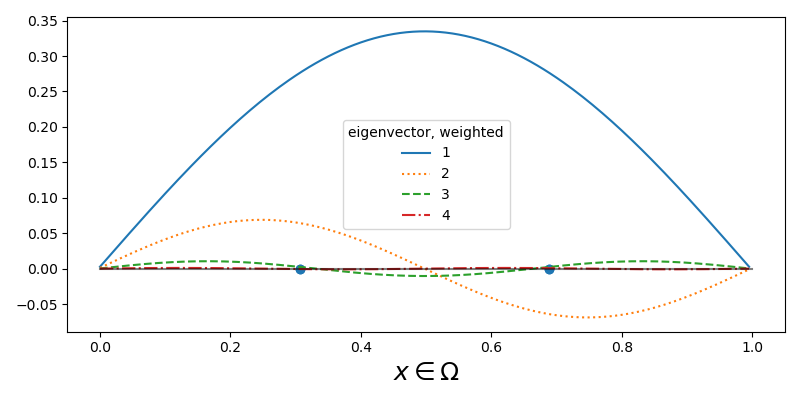
\includegraphics[width=\textwidth]{../latex/figs/eigenvectors_dst_scaled.png}
    \caption{D-optimal measurement locations ($m=4$ measurements) and
      weighted eigenvectors for finding the initial condition of the
      1D heat equation. Measurement locations and weighted
      eigenvectors are plotted over the computational domain $\Omega =
      [0, 1]$ (x-axis). Measurement clusterization occurs
      approximately at $0.31$ and $0.69$. These two locations are a
      compromise between the amplitudes of the first and second
      eigenvectors, which are the eigenvectors that a D-optimal design
      aims to measure. Allocating $m=4$ measurements into two
      locations results in clusterization, according to the pigeonhole
      principle.}
  \label{fig:why}
\end{figure}



%% \begin{quote}
%%   Building on Theorem \ref{thm:char}, we can now give a compelling
%%   explanation to the measurement clusterization we observed for the
%%   inverse problem of the heat equation, see Section
%%   \ref{subsub:clusterization1} below. We also suggest a generic
%%   explanation for clusterization, see Section
%%   \ref{subsub:clusterization2}.
%%   \newline
%%   \newline
%%   Consider $\fwd$ and $\prcov$ from \emph{the inverse problem of the
%%   heat equation}. As before, we denote the eigenvalues of
%%   $\fwd\prcov\fwd^*$ by $\lambda_j$. We input these eigenvalues into
%%   our \emph{generic} model, and find a D-optimal design $\opt$ for our
%%   generic model using Theorem \ref{thm:char}. In our generic model,
%%   the measurements we take are best utilized in reducing uncertainty
%%   for the first $k$ eigenvectors. So, a D-optimal design arising from
%%   our \emph{generic model} completely avoids measuring eigenvectors
%%   $k+1$ and above.
%%   \newline
%%   \newline
%%   Of course, in a real life problem --- such as the inverse problem of
%%   the 1D heat equation --- it is likely impossible to find measurement
%%   locations for which all eigenvectors $k+1$ and above are
%%   zero. However, if the eigenvalues of $\fwd\prcov\fwd^*$ decay
%%   quickly (recall the square-exponential decay for eigenvalues of the
%%   1D heat equation in eq.\eqref{eq:decay}), a D-optimal design will
%%   try to balance measuring a small number (i.e.~$k$) of the leading
%%   eigenvectors.
%% \end{quote}
%% \begin{quote}
%%   The abovementioned balance is explored in
%%   Fig.~\ref{fig:eigenvectors}. We allow $m=4$ measurements in $\Omega
%%   = [0,1]$ and observe that D-optimal measurement locations are
%%   clustered at $x_1 = 0.31$ and $x_2 = 0.69$. Upon close inspection of
%%   the scaled eigenvectors of $\fwd \prcov \fwd^*$, we first observe
%%   that eigenvectors $3$ and above have negligible prior
%%   amplitude. Since we only have $m=4$ measurements at our disposal, we
%%   interpret these results, following Theorem \ref{thm:char}, as
%%   implying we should only care about measuring the first and second
%%   eigenvectors. Then, we note the D-optimal $x_1,x_2$ present a
%%   compromise between the amplitude of the first and second
%%   eigenvectors. For example, a measurement at $x=0.5$ would have
%%   ignored the second eigenvector altogether, since the second
%%   eigenvector is zero at $x=0.5$.
%%   \newline
%%   \newline
%%   Now we can understand measurement clusterization for the inverse
%%   problem of the heat equation. A D-optimal design attempts to measure
%%   the first $k$ eigenvectors of $\fwd \prcov \fwd^*$. But there may be
%%   (spatial) limitations on where these $k$ eigenvectors have large
%%   amplitude. For the inverse problem of the heat equation there are
%%   two spatial locations that present a good compromise between the
%%   amplitudes of the first and second eigenvectors, namely $x_1$ and
%%   $x_2$ --- see Fig.~\ref{fig:eigenvectors}. We have $m=4$
%%   measurements at our disposal but only two spatial locations that are
%%   a good compromise between the first and second scaled
%%   eigenvectors. Thus, clusterization arises as a consequence of the
%%   pigeonhole principle.
%% \end{quote}

%% \begin{figure}\label{fig:eigenvectors}
%%   \centering
%%   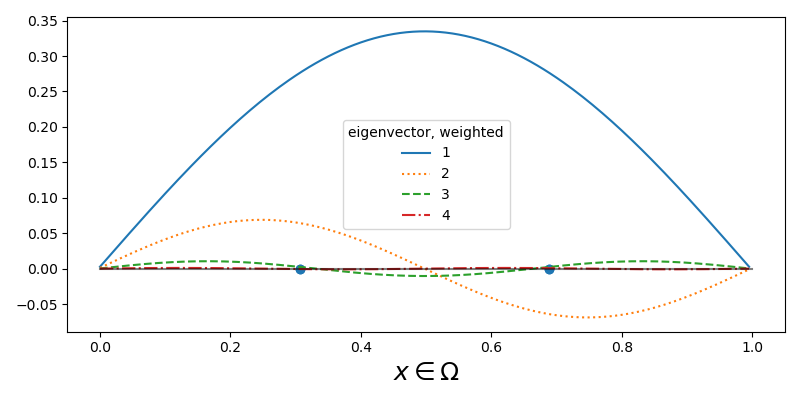
\includegraphics[width=\textwidth]{../latex/figs/eigenvectors_dst_scaled.png}
%%   \caption{D-optimal measurement locations ($m=4$ measurements) and
%%     weighted eigenvectors for finding the initial condition of the 1D
%%     heat equation. Measurement locations and weighted eigenvectors are
%%     plotted over the computational domain $\Omega = [0, 1]$
%%     (x-axis). Measurement clusterization occurs approximately at
%%     $0.31$ and $0.69$. These two locations are a compromise between
%%     the magnitudes of the first and second eigenvectors, which are the
%%     eigenvectors that a D-optimal design aims to measure. Allocating
%%     $m=4$ measurements into two locations results in clusterization,
%%     according to the pigeonhole principle.}
%%   \label{fig:why}
%% \end{figure}
 

